\documentclass[fr]{../../../eplnotes}

\usepackage{float}
\usepackage{../../../eplmath}


\hypertitle{Mathématiques discrètes I : Théorie et algorithmique des graphes}{5}{INMA}{1691}
{Gilles Peiffer}
{Raphaël Jungers}[
\paragraph{Remarque} Ce document reprend les notes prises
au cours de l'année 2018-2019.
]

\section{Premier cours magistral}
\subsection{Introduction}
	De façon informelle,
	on peut dire qu'un graphe
	est ``un réseau de sommets reliés par des arêtes''.
	Un exemple d'un graphe serait donc par exemple
	celui à la \figuref{graph}.
	\begin{figure}[H]
	\centering
	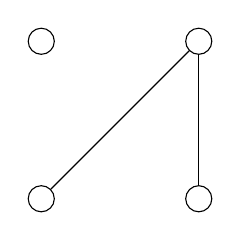
\begin{tikzpicture}
		\node[draw, circle] at (-1,2)  (1) {};
		\node[draw, circle] at ( 1,2)  (2) {};
		\node[draw, circle] at (-1,0)  (3) {};
		\node[draw, circle] at ( 1,0)  (4) {};

		\draw[-] (2) edge node[anchor = north] {} (3);
		\draw[-] (2) edge node[anchor = north east] {} (4);
	\end{tikzpicture}
	\caption{Un graphe à 4 sommets et 2 arêtes.}
	\label{fig:graph}
	\end{figure}

	Pourquoi est-il intéressant d'étudier la théorie des graphes?
	Grâce aux résultats de celle-ci,
	énormément de problèmes semblant initialement compliqués
	sont réduits à des problèmes relativement simples.
	En effet, un acronyme intéressant,
	très souvent valable en théorie des graphes,
	est \textsc{TONCAS}:
	``\emph{The Obviously Necessary Condition is Also Sufficient}'',
	c'est-à-dire que si une condition paraît intuitivement nécessaire,
	il y a de bonnes chances qu'elle soit également suffisante.
\subsection{Définitions}
	\begin{mydef}[Graphe]
		Un \emph{graphe} $G$ est un triplet ordonné $(V, E, \psi)$, où:
		\begin{itemize}
		\item $V$ est un ensemble dont les éléments sont appelés sommets ou noeuds;
		\item $E$ est un ensemble dont les éléments sont appelés arêtes;
		\item $\psi$ est une fonction, dite fonction d'incidence,
		qui associe à chaque arête un sommet ou une \emph{paire} de sommets.
		\end{itemize}
	\end{mydef}
	Prenons de nouveau un exemple de graphe (\figuref{graph_2}).
	\begin{figure}[H]
	\centering
	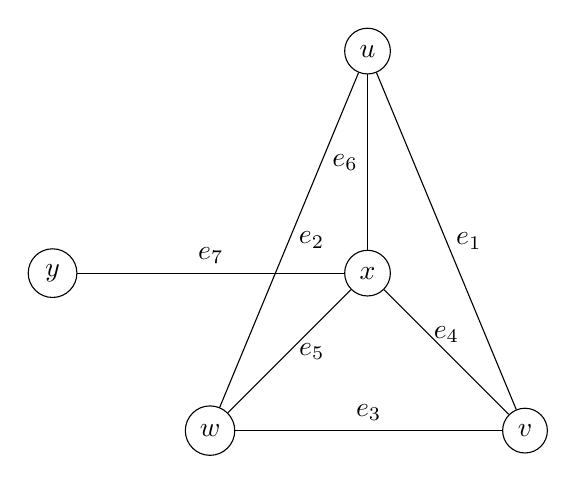
\begin{tikzpicture}
		\node[draw, circle] at ( 0, 2.82)  (u) {$u$};
		\node[draw, circle] at ( 0, 0  )  (x) {$x$};
		\node[draw, circle] at (-4, 0  )  (y) {$y$};
		\node[draw, circle] at ( 2,-2  )  (v) {$v$};
		\node[draw, circle] at (-2,-2  )  (w) {$w$};

		\draw (u) -- (v) node [midway, right] {$e_1$};
		\draw (u) -- (w) node [midway, right] {$e_2$};
		\draw (v) -- (w) node [midway, above] {$e_3$};
		\draw (x) -- (v) node [midway, above] {$e_4$};
		\draw (x) -- (w) node [midway, right] {$e_5$};
		\draw (x) -- (u) node [midway, left] {$e_6$};
		\draw (x) -- (y) node [midway, above] {$e_7$};
	\end{tikzpicture}
	\caption{Un graphe à 5 sommets et 7 arêtes.}
	\label{fig:graph_2}
	\end{figure}
	Pour ce graphe, on a
	\begin{align*}
		V &= \{u, v, w, x, y\}\,,\\
		E &= \{e_1, e_2, \dots, e_7\}\,,\\
		\psi(e_1) &= (u,v)\,,\\
		\psi(e_2) &= (u,w)\,,\\
		&\vdotswithin{=}\\
		\psi(e_7) &= (x,y)\,.\\
	\end{align*}

	\begin{mydef}[Degré]
		Le degré d'un sommet
		est le nombre d'arêtes incidentes à celui-ci.
	\end{mydef}

	\begin{myexem}[Sous-graphe]
		Un exemple de sous-graphe du graphe en \figuref{graph_2}
		est le graphe en \figuref{subgraph}.
		\begin{figure}[H]
		\centering
		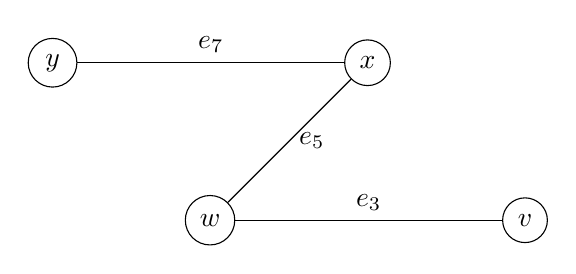
\begin{tikzpicture}
			\node[draw, circle] at ( 0, 0  )  (x) {$x$};
			\node[draw, circle] at (-4, 0  )  (y) {$y$};
			\node[draw, circle] at ( 2,-2  )  (v) {$v$};
			\node[draw, circle] at (-2,-2  )  (w) {$w$};
			\draw (v) -- (w) node [midway, above] {$e_3$};
			\draw (x) -- (w) node [midway, right] {$e_5$};
			\draw (x) -- (y) node [midway, above] {$e_7$};
		\end{tikzpicture}
		\caption{Un graphe chemin à 4 sommets et 3 arêtes,
		sous-graphe de celui à 5 sommets et 7 arêtes en \figuref{graph_2}.}
		\label{fig:subgraph}
		\end{figure}
		En général, un \emph{sous-graphe} du graphe $(V, E, \psi)$
		est un graphe $(V', E', \psi')$ avec :
		\begin{itemize}
		\item $V' \subseteq V$;
		\item $E' \subseteq E$;
		\item $\psi'$ est la restriction de $\psi$ à $E'$.
  \end{itemize}
	\end{myexem}

	\begin{mydef}[Graphe simple]
		Un graphe simple est un graphe sans boucle ni arête multiple.
	\end{mydef}

	Il faut noter qu'un graphe est une notion abstraite,
	indépendante de sa représentation.
	Le graphe $G$ aurait tout aussi bien pu être noté sous la forme
	\begin{figure}[H]
	\centering
	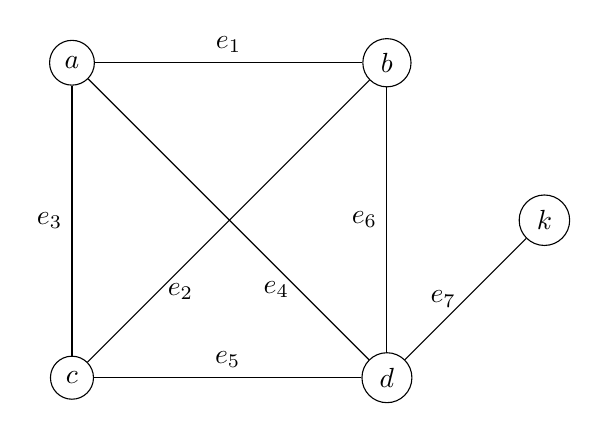
\begin{tikzpicture}
		\node[draw, circle] at ( 2, 2)  (u) {$b$};
		\node[draw, circle] at ( 2,-2)  (x) {$d$};
		\node[draw, circle] at ( 4, 0)  (y) {$k$};
		\node[draw, circle] at (-2, 2)  (v) {$a$};
		\node[draw, circle] at (-2,-2)  (w) {$c$};

		\draw (u) -- (v) node [midway, above] {$e_1$};
		\draw (u) -- (w) node [near end, right] {$e_2$};
		\draw (v) -- (w) node [midway, left] {$e_3$};
		\draw (x) -- (v) node [near start, left] {$e_4$};
		\draw (x) -- (w) node [midway, above] {$e_5$};
		\draw (x) -- (u) node [midway, left] {$e_6$};
		\draw (x) -- (y) node [midway, left] {$e_7$};
	\end{tikzpicture}
	\caption{Le graphe de la \figuref{graph_2} représenté différemment.}
	\label{fig:graph_2_iso}
	\end{figure}

	L'\emph{isomorphisme} est
	\[
	\begin{array}{cc}
		y & k \\
		x & d \\
		w & c \\
		u & b \\
		v & a
	\end{array}
	\]

	\subsection{Isomorphisme de graphes}
	\begin{mydef}[Isomorphisme de graphes]
		Deux graphes $(V, E, \psi)$ et $(V', E', \psi')$
		sont dits \emph{isomorphes} s'il existe
		des bijections $f \colon V \to V'$ et $g \colon E \to E'$ telles que:
		\[
		\psi(e) = (u,v) \iff \psi(g(e)) = \big(f(u),f(v)\big)\,.
		\]
		Deux graphes sont isomorphes
		s'il y a une bijection entre les n\oe{}uds et les arêtes.
	\end{mydef}

	\begin{mypropo}[La relation d'isomorphisme est une relation d'équivalence]
		Toute relation d'équivalence satisfait à 3 conditions:
		\begin{itemize}
			\item elle est réflexive;
			\item elle est symétrique;
			\item elle est transitive.
		\end{itemize}
		Prouvons que la relation d'isomorphisme de graphes
		est une relation d'équivalence.
		\begin{proof}
			Commençons par prouver la réflexivité.
			Cela revient à dire qu'il y a un isomorphisme
			entre le graphe et lui-même.
			Pour prouver cela,
			il suffit de remarquer
			qu'un isomorphisme satisfaisant cette propriété
			est la permutation identité,
			car elle satisfait $G_1 \simeq G_2$.
			\bigbreak
			Prouvons maintenant la symétrie de l'isomorphisme.
			Soit $f \colon V(G_1) \to V(G_2)$,
			alors $f^{-1}$ est un isomorphisme de $G_2 \to G_1$.
			En effet, on sait que
			\[
			uv \in E(G_1) \iff f(u)f(v) \in E(G_2)\,.
			\]
			On sait alors que $\forall x,y \in V(G_2)$
			\[
			f^{-1}(x)f^{-1}(y) \in E(G_1) \iff xy \in E(G_2)\,.
			\]
			\bigbreak
			Finalement, prouvons la transitivité.
			Supposons que $f \colon V(F) \to V(G)$
			et $g \colon V(G) \to V(H)$.
			On a alors
			\begin{align*}
				uv \in E(F) &\iff f(u)f(v) \in E(G)\\
				\intertext{et}
				f(u)f(v) \in E(G) &\iff g\big(f(u)\big)g\big(f(v)\big) \in E(H)\,.
			\end{align*}
			Cela implique que $g \circ f$
			est une bijection,
			ce qui implique à son tour $F \simeq H$.
			\bigbreak
			En combinant ces trois résultats,
			on remarque donc que l'isomorphisme de graphes
			est une relation d'équivalence.
		\end{proof}
	\end{mypropo}

	\begin{mypropo}[$G \simeq H \iff \widebar{G} \simeq \widebar{H}$]
		La preuve est immédiate en observant
		que toute non-arête de $G$ sera également
		une non-arête de $H$.
		Ce petit truc permet parfois
		de voir relativement facilement
		si deux graphes sont isomorphes,
		bien qu'en général,
		cela reste une tâche compliquée.
		% TODO add graphs
	\end{mypropo}
	\subsection{Théorème d'Euler}
	Un des nombreux théorèmes dus à Leonhard Euler
	est l'observation qu'un graphe connexe est eulérien
	si et seulement si le degré de tous ses sommets est pair.
	\begin{mytheo}[Théorème d'Euler]
		Un graphe connexe est eulérien
		si et seulement si le degré de chacun de ses sommets
		est un nombre pair.
		\begin{proof}
		Démontrons l'implication directe d'abord.
		Considérons le problème eulérien
		où en tout n\oe{}ud il y a
		autant d'arêtes entrantes que sortantes.
		(Il s'agit de la condition pour qu'un graphe soit eulérien.)
		Le degré du n\oe{}ud est
		la somme de ce nombre d'arêtes entrantes et sortantes.
		Il sera donc égal à $2n$,
		où $n$ est le nombre d'arêtes entrantes,
		ce qui est toujours un nombre pair.
		\bigbreak
		L'implication indirecte se démontre par construction,
		et se comprend intuitivement par construction.\footnote{C'est vague comme preuve,
		mais il y en a des plus complètes sur Internet,
		notamment dans le syllabus en ligne.}
		\end{proof}
	\end{mytheo}
\section{Deuxième cours magistral}
\subsection{Représentations d'un graphe}
Soit le graphe $G$ de la \figuref{mat}.
\begin{figure}[H]
	\centering
	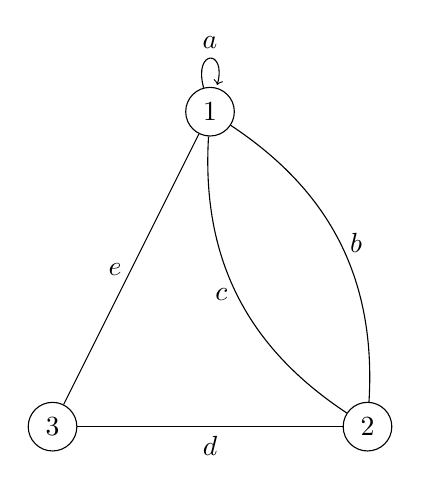
\begin{tikzpicture}
	\node[draw, circle] at ( 0, 4)  (1)  {$1$};
	\node[draw, circle] at ( 2, 0)  (2)  {$2$};
	\node[draw, circle] at (-2, 0)  (3)  {$3$};

	\draw[-] (1) edge [loop above] node {$a$} (1);
	\draw[-] (1) edge [bend left] node [midway,right] {$b$} (2);
	\draw[-] (1) edge [bend right] node [midway,left] {$c$} (2);
	\draw[-] (2) edge node [midway,below] {$d$} (3);
	\draw[-] (1) edge node [midway,left] {$e$} (3);
	\end{tikzpicture}
	\caption{Un graphe.}
	\label{fig:mat}
\end{figure}
On peut représenter ce graphe de deux façons distinctes:
\begin{itemize}
	\item sa \emph{matrice d'incidence} et
	\item sa \emph{matrice d'adjacence}.
\end{itemize}
\begin{mydef}[Matrice d'incidence d'un graphe non orienté]
	La matrice d'incidence d'un graphe non orienté
	est la matrice rectangulaire $M$ de taille $n \times m$
	dont l'élément $m_{ij}$ est
	\begin{itemize}
		\item $1$ si le sommet $v_i$ est une extrémité de l'arête $e_j$;
		\item $2$ si l'arête $x_{j}$ est une boucle sur $v_{i}$;
		\item $0$ sinon.
	\end{itemize}
\end{mydef}
\begin{mydef}[Matrice d'adjacence]
	La matrice d'adjacence d'un graphe $G$ à $n$ sommets
	est la matrice $n \times n$ booléenne $A$
	dont l'élément $a_{ij}$ est
	\begin{itemize}
		\item $1$ si $v_i v_j \in E$;
		\item $0$ sinon.
	\end{itemize}
\end{mydef}
\bigbreak
Pour le graphe $G$ de la \figuref{mat},
on a donc les représentations suivantes:
\[
A = \bordermatrix{  & 1 & 2 & 3 \cr
                  1 & 1 & 2 & 1 \cr
                  2 & 2 & 0 & 1 \cr
                  3 & 1 & 1 & 0 \cr}\,,
\quad
M = \bordermatrix{  & a & b & c & d & e\cr
                  1 & 2 & 1 & 1 & 0 & 1\cr
                  2 & 0 & 1 & 1 & 1 & 0\cr
                  3 & 0 & 0 & 0 & 1 & 1\cr}\,.
\]

\begin{mytheo}[Théorème des poignées de main]
	La somme des degrés des n\oe{}uds d'un graphe
	est deux fois le nombre d'arêtes.
	Mathématiquement,
	\[
	\sum_{v_i \in V} \deg(v_i) = 2 \abs{E}\,.
	\]
	\begin{proof}
		\begin{align*}
		\sum_{i}\sum_{j} M_{ij} &= \sum_{v_i \in V} \deg(v_i)\\
		&= \sum_j 2\\
		&= 2 \abs{E}\,.
		\end{align*}
	\end{proof}
\end{mytheo}

\begin{mytheo}[Matrice d'adjacence et nombre de parcours]
	Soit $A$ la matrice d'adjacence d'un graphe.
	Alors l'élément $a^k_{ij}$ de $A^k$ ($k \ge 0$)
	est le nombre de parcours de longueur $k$
	de $v_i$ vers $v_j$.
	\begin{proof}
		Par induction.
		\begin{description}
			\item[Cas de base.]
			Pour $k = 1$, c'est vrai
			par la définition de la matrice d'adjacence.
			\item[Cas inductif.]
			Supposons la propriété vraie pour $k$.
			Soit
			\begin{itemize}
				\item $i$ et $j$ deux n\oe{}uds,
				\item $\pi^{k+1}_{ij}$ le nombre de parcours
				de $i$ vers $j$ de longueur $k+1$,
				\item  $\epsilon_{ij}$ le nombre d'arêtes
				de $i$ vers $j$ et
				\item $a^k_{ij}$ l'entrée en ligne $i$
				et colonne $j$ de $A^k$.
			\end{itemize}
			On a alors
			\begin{align*}
			\pi^{k+1}_{ij} &= \sum_{l \in V} \pi_{il}^{k} \epsilon_{lj}\\
			&= \sum_{l \in V} a^k_{il} a_{lj}\\
			&= a^{k+1}_{ij}\,.
			\end{align*}
		\end{description}
	\end{proof}
\end{mytheo}

\begin{myexem}
\label{exem:code}
Un autre exemple d'utilisation de la matrice d'adjacence
est qu'elle permet par exemple de répondre à la question
``Combien de mots binaires de longueur $k$ ne contiennent pas `$111$'?''\,.

Prenons le graphe du problème (\figuref{code}),
où chaque n\oe{}ud est la terminaison actuelle du mot,
et où chaque arête indique la terminaison que l'on aurait
en rajoutant soit un $0$ soit un $1$.
\begin{figure}[H]
	\centering
	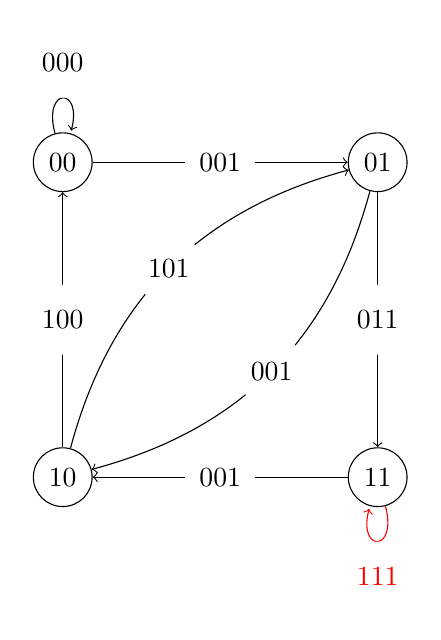
\begin{tikzpicture}
	\node[draw, circle] at (-2, -2)  (10)  {$10$};
	\node[draw, circle] at (-2,  2)  (00)  {$00$};
	\node[draw, circle] at ( 2,  2)  (01)  {$01$};
	\node[draw, circle] at ( 2, -2)  (11)  {$11$};

	\begin{scope}[every node/.style={fill=white,circle}]
		\path[->] (00) edge [loop above] node {$000$} (00);
		\path[->] (11) edge [loop below,red] node {$111$} (11);
		\path[->] (00) edge node {$001$} (01);
		\path[->] (10) edge node {$100$} (00);
		\path[->] (10) edge [bend left] node {$101$} (01);
		\path[->] (01) edge [bend left] node {$001$} (10);
		\path[->] (01) edge node {$011$} (11);
		\path[->] (11) edge node {$001$} (10);
	\end{scope}
	\end{tikzpicture}
	\caption{Graphe de l'Exemple~\ref{exem:code}.
	La seule arête qu'on ne compte pas est celle en rouge,
	car c'est ce cas-là qu'on veut éviter.}
	\label{fig:code}
\end{figure}
On construit la matrice d'adjacence (en ne comptant pas l'arête rouge):
\[
A = \begin{pmatrix}
1 & 1 & 0 & 0\\
0 & 0 & 1 & 1\\
1 & 1 & 0 & 0\\
0 & 0 & 1 & 0
\end{pmatrix}\,.
\]
Maintenant, en calculant les valeurs propres de la matrice $A$,
et en choisissant la plus grande ($\rho \approx 1.84$ en l'occurrence),
on peut trouver la capacité du code.
Pour une longueur $k$,
le nombre de mots ne contenant pas la séquence $111$ est $\approx \rho^k$.
\end{myexem}
\subsection{Graphe biparti}
\begin{mytheo}[Graphe biparti]
\label{theo:bipartite}
	Un graphe est biparti si et seulement si
	tous ses cycles sont de longueur paire.
	\begin{proof}
	\noindent
	\newline
	$\boxed{\implies}$
	\newline
	Soit un graphe $G$ biparti et un cycle $C = v_0, v_1, v_2, \dots, v_0$.
	Supposons $v_0 \in V_0$, $v_1 \in V_1$, $v_2 \in V_0$,\dots.
	Tout cycle termine en $V_0$ et contient donc
	un nombre pair d'arêtes.

	\noindent
	\newline
	$\boxed{\impliedby}$
	\newline
	Soit $v_0$ un n\oe{}ud arbitraire.
	On définit
	\begin{align*}
		V_0 &= \set{v \suchthat d(v,v_0) \textnormal{ est pair}}\\
		V_1 &= \set{v \suchthat d(v,v_0) \textnormal{ est impair}}\,.
	\end{align*}
	Par contradiction.
	Supposons sans perte de généralité $\exists u,v \in V_0$.
	Soient $p,q$ les plus courts chemins
	de $v_0$ à $u$ et $v$ respectivement.
	\begin{figure}[H]
	\centering
	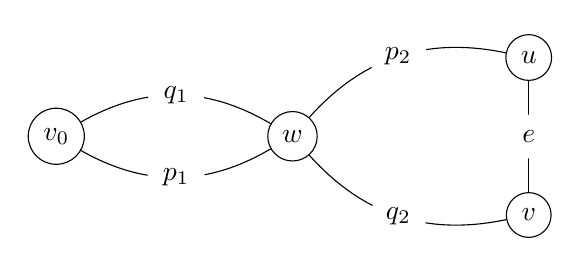
\begin{tikzpicture}
	\begin{scope}[every node/.style={fill=white,circle}]
		\node[draw, circle] at (-4, 0)  (v0)  {$v_0$};
		\node[draw, circle] at (-1, 0)  (w)  {$w$};
		\node[draw, circle] at ( 2, 1)  (u)  {$u$};
		\node[draw, circle] at ( 2,-1)  (v)  {$v$};

		\draw[-] (v0) edge [bend left]  node {$q_1$} (w);
		\draw[-] (v0) edge [bend right] node {$p_1$} (w);
		\draw[-] (w) edge [bend left]  node {$p_2$} (u);
		\draw[-] (w) edge [bend right] node {$q_2$} (v);
		\draw[-] (u) edge node {$e$} (v);
	\end{scope}
	\end{tikzpicture}
	\caption{Le graphe pour la preuve du Théorème~\ref{theo:bipartite}.}
	\label{fig:bipartite}
	\end{figure}
	Soit $w$ le dernier n\oe{}ud dans $p \cap q$.
	Notre \emph{claim} est que $p_2 e q_2$ est un cycle pair.
	Cependant,
	\begin{align*}
	\abs{p_1 p_2 e q_2 q_1} &= \abs{p_1} + \abs{p_2 e q_2} + \abs{q_1}\\
	d(v_0,u) + d(v_0,v) + 1 &= 2 \abs{p_1} + \abs{p_2 e q_2}\,.
	\end{align*}
	Comme le coté de gauche de cette équation est impair
	($u$ et $v$ sont à une distance paire de $v_0$ car ils sont dans $V_0$),
	et que $2 \abs{p_1}$ est évidemment pair,
	le cycle $p_2 e q_2$ doit être impair.
	C'est donc une contradiction,
	ce qui termine la preuve.
	\end{proof}
\end{mytheo}
\begin{mytheo}[Théorème de l'amitié]
	% TODO 
\end{mytheo}

\end{document}
